\section{Case Study}
\label{sec:case}

%%\wrm{Re-do case studies in Bud} \wrm{Break cart development down into
%%iterations} \wrm{How does the language naturally lead us to an order
%%independent style?  Talk about inserting all sorts of exotic stuff like queues
%%if we want a highly order-dependent imperative style.}

\jmh{We discussed the following on the phone.  (1) Handle shopping in two styles: destructive updates, and disorderly accumulation of increment/decrement.  (2) Do analysis on them to detect need for coordination in only the first, show that (annotated) 2PC removes the compiler warning.  (3) Deploy destructive+2PC on EC2 and show practical benefits of avoiding coordination.  (4) Evolve the program with new rules for checkout and/or inventory, show how the disorderly version is no longer monotonic.  Fix that  with 2PC where needed.  Also make sure the destructive version works with the new rules.  Now show that the disorderly version is still better than the destructive one, by coordinating only where needed.}

\jmh{Finally, show what would happen if you didn't coordinate the inventory bit, but tracked taint.  Note that tainted output is the stuff where programmers need to write compensation logic.}


In this section, we implement two different styles of distributed shopping cart
applications in Bud.  First, we implement a ``destructive,'' overwriting
shopping cart application using a simple key-value store implemented in Bud.
Second, we implement a ``disorderly'' cart which accumulates updates in a 
set-wise fashion and describes how to combine the updates into a final result.

For each, we apply whole-program analysis techniques to discover points of 
order in the program.  The analysis, based on traditional stratification
techniques, represents the dependency graph of predicates (and hence the 
flow of tuples) as a staged dataflow graph.  Asynchronous message sending
is indicated by a dotted line in the graph, while edges that involve 
nonmonotonic logic are marked with a $\lnot$.  Edges that involve a temporal 
edge are marked with a $+$.  Strongly connected components having both a $\lnot$ and a $+$ edge are grouped into temporal clusters.  Individual monotonic components 
(or strata) are surrounded by a dashed rectangle.  A point of order occurs
wherever an edge crosses strata, or at any self-edge attached to a temporal cluster.

To resolve a point of order, the programmer may add coordination logic.
As we observe in Section~\ref{sec:calm}, waiting requires counting and coordination code almost always 
requires nonmonotonic logic, so the augmented program is not reanalyzed.
Instead, coordination code is always associated with an annotation that can
be interpreted as a contract about a point of order.  Such contracts will
typically guarantee an ordering over arriving tuples, or guarantee a 
a barrier-passing condition (indicating that there will be no more tuples).

\begin{comment}
\begin{figure}[t]
\begin{tiny}
\begin{verbatim}
class BudKVS < BestEffortDelivery
#class BudKVS < ReliableDelivery
  def state
    super
    table :bigtable, ['key'], ['value']
    #table :stor_saved, ['client', 'server', 'key', 'reqid', 'value']
    table :stor_saved, ['server','client', 'key', 'reqid', 'value']
    table :member, ['peer']
    scratch :kvstore, ['server', 'client', 'key', 'reqid'], ['value']
  end

  declare
    def kstore
      readback = join [stor_saved, pipe_out], [stor_saved.reqid, pipe_out.id]
      stor_saved <- readback.map{ |s, p| s }
      stor_saved <+ kvstore.map{|k| k}
      bigtable <+ readback.map { |s, p| [s.key, s.value] }

      jst = join [bigtable, stor_saved, pipe_out], [bigtable.key, stor_saved.key], [stor_saved.reqid, pipe_out.id]
      bigtable <- jst.map { |b, s, p| b }
    end

  declare
    def replicate
      jrep = join [kvstore, member]
      pipe <+ jrep.map do |s, m|
        if m.peer != @addy and m.peer != s.client
          [m.peer, @addy, s.reqid, [s.key, s.value]]
        end
      end
  
      kvstore <+ pipe_chan.map do |p|
        if @addy == p.dst and p.dst != p.src
          [p.dst, p.src, p.payload.index(0), p.id, p.payload.index(1)] 
        end
      end

      # bootstrap slaves: they are not required to replicate data to the source.
      pipe_out <= jrep.map { |s, m| [m.peer, @addy, s.reqid, [s.key, s.value]] if s.client == m.peer }
    end

end


\end{verbatim}
\vspace{-10pt}
\caption{An agent sends a constrained promise if it has voted for an
  update in a previous view.}
\label{fig:anchor}
\end{tiny}
\vspace{-2pt}
\end{figure}

\end{comment}

\subsection{Destructive Cart}

\begin{figure}[t]
\begin{tiny}
\begin{verbatim}
  declare def accumulate
      kvstore <= iaction.map do |a| 
        unless bigtable.map{|b| b.key}.include? a.session
          if a.action == "A"
            [a.server, a.client, a.session, Array.new.push(a.item)]
          elsif a.action == "D"
            [a.server, a.client, a.session, Array.new]
          end
        end
      end
  end

  declare def consider
      joldstate = join [bigtable, iaction], [bigtable.key, iaction.session]
      kvstore <= joldstate.map do |b, a| 
       if a.action == "A"
          [a.server, a.client, a.session, b.value.push(a.item)]
        elsif a.action == "D"
          copy = b.value.clone;
          copy.delete_at(copy.index(a.item));
          [a.server, a.client, a.session, copy]
        end
      end
      response <+ join([bigtable, checkout], [bigtable.key, checkout.session]).map do |s, c|
        [c.client, c.server, s.key, s.value]
      end
  end


\end{verbatim}
\end{tiny}
\centering
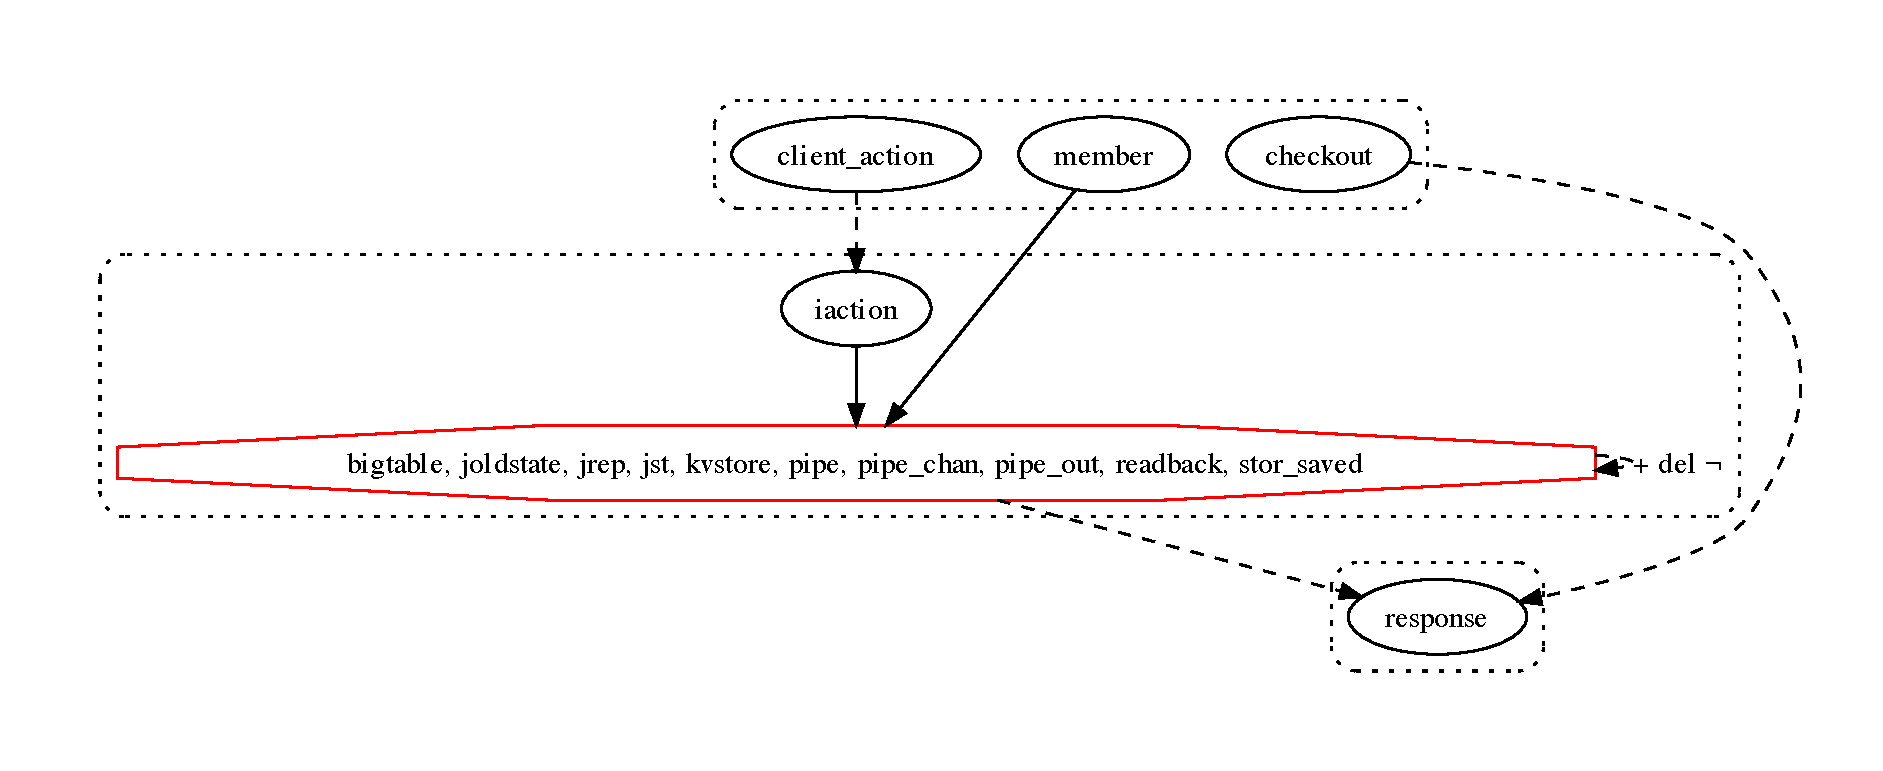
\includegraphics[width=0.9\linewidth]{fig/ImperativeCartServer_gvoutput.pdf}

\caption{Destructive Cart (cycles collapsed)}
\label{fig:pdg-destructive}
\end{figure}

Figure~\ref{fig:pdf-destructive} shows the destructive shopping cart code
and its accompanying analysis.  Note the points of order between \emph{client\_action} and \emph{iaction}
and between the temporal cluster and itself.  This means that the arrival 
timing and order of tuples crossing the point of order may result in different
end results.  Although there is no obvious nonmonotonicity in the destructive
cart code as shown, the underlying key-value store uses updateable state
to implement the storage of opaque, mutable values of keys, and our global
analysis detects this.
To ensure a consistent final state across all replicas, We may require coordination
between client and server at every update to the cart, and between the 
server and all replicas at each update.  

We can easily achieve this without modfying the cart implementation
by redefining the key-value store to extend
ReliableDelivery or, better, QuorumDeliver instead of BestEffortDelivery, and require acknowledgement from a server or a quorum of servers, respectively.
The simplest (and least performant) approach is to require unanimous quorum,
approximating ``eager replication''~\cite{dangers} via two-phase commit.


\subsection{Disorderly Cart}

\begin{figure}[t]
\begin{tiny}
\begin{verbatim}
  declare def accumulate 
      cart_action <= action.map { |c| [c.session, c.item, c.action, c.reqid] }
      action_cnt <= cart_action.group([cart_action.session, 
          cart_action.item, cart_action.action], count(cart_action.reqid))
      action_cnt <= cart_action.map do |a| 
        unless cart_action.map{|c| [c.session, c.item] if c.action == "D"}.include? [a.session, a.item] 
           [a.session, a.item, 'D', 0]
        end 
      end
  end

  declare def consider
      status <= join([action_cnt, action_cnt, checkout]).map do |a1, a2, c| 
        if a1.session == a2.session and a1.item == a2.item 
            and a1.session == c.session and a1.action == "A" and a2.action == "D"
           [a1.session, a1.item, a1.cnt - a2.cnt] if (a1.cnt - a2.cnt) > 0
        end
      end
      response <= join([status, checkout], [status.session, checkout.session]).map do |s, c| 
        [c.client, c.server, s.session, s.item, s.cnt]
      end
    end

  declare def replicate
      action <+ join([action, member]).map do |a, m|
          [m.player, a.server, a.session, a.item, a.action, a.reqid]
      end

      checkout <+ join([checkout, member]).map do |c, m|
         [m.player, c.client, c.session]
      end
    end


\end{verbatim}
\end{tiny}

\centering
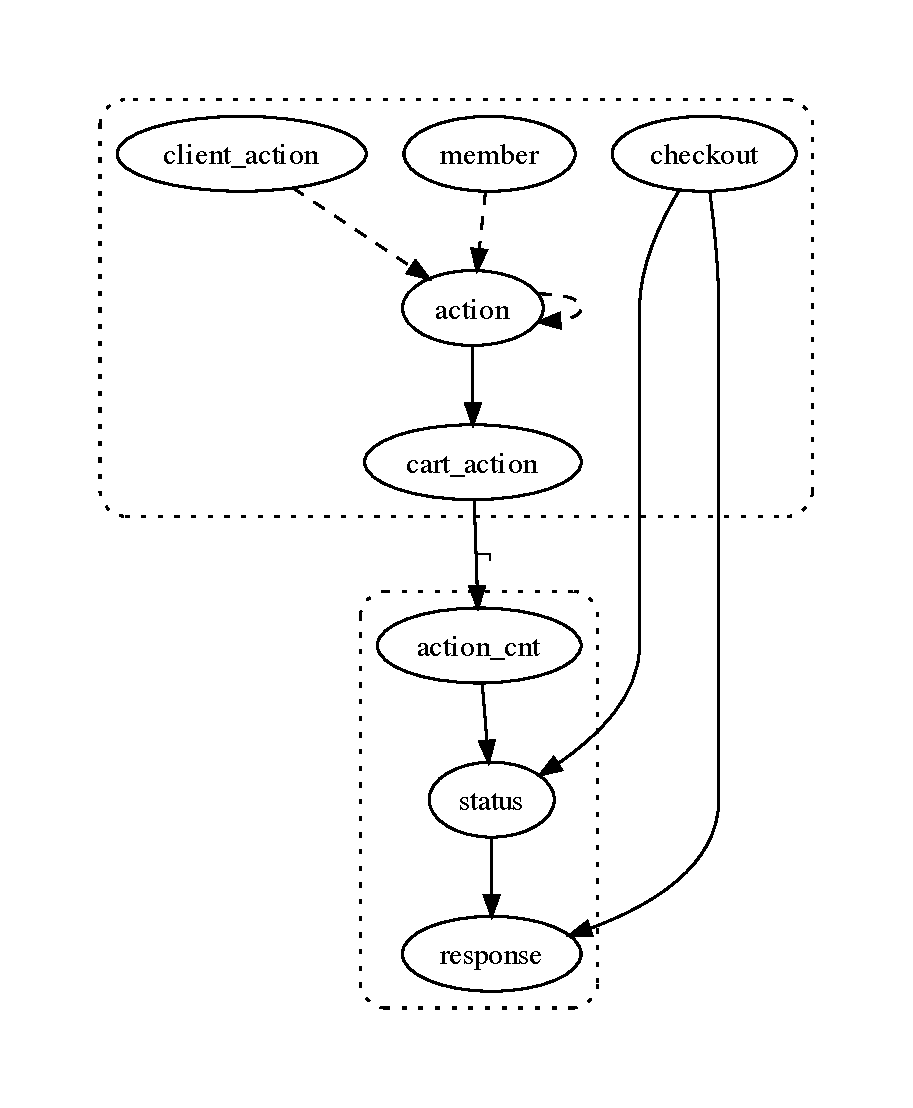
\includegraphics[width=0.7\linewidth]{fig/BasicCartServer_gvoutput.pdf}
\caption{Disorderly Cart}
\label{fig:pdg-disorderly}
\end{figure}


Figure~\ref{fig:pdg-disorderly} shows the ``disorderly'' cart and analysis.
Dotted lines indicate that 
\emph{action} (owned by the server) is derived from \emph{client\_action} 
(owned by the client) via an asynchronous message, and that \emph{action} 
derives itself via messages when it is replicated.  However, the analysis
shows that because these derivations are strictly monotonic, no points of
order are crossed.  Hence, clients may send and servers may replicate 
updates without any coordination: regardless of timing and ordering, the end
result will be the same.

The analysis does indicate a point of order at checkout, when a \emph{checkout}
message is joined with an aggregate over the set of updates.  While the 
accumulation of state has been monotonic, summarization of the cart state
requires us to assume (or prove) that there will be no further updates.



